\documentclass{acm_proc_article-sp}

\usepackage{natbib}
\usepackage{url}

\makeatletter
\def\@copyrightspace{\relax}
\makeatother

\begin{document}

\title{SMS Immunization Manager (SIM)}

\numberofauthors{4} 
\author{
       % \alignauthor
       Jenny Kang, Isaac Reynolds, Jackson Roberts, Nicholas Shahan\\
              \affaddr{University of Washington}\\
              \affaddr{Seattle, WA, USA}\\
              \email{jskang, isaacr, jcwr, nshahan@uw.edu}
}

\maketitle
\begin{abstract}
There is a great need for timely and accurate reports in order to facilitate the efficient distribution of vaccines across health centers within a country. The SMS Immunization Manager (SIM) is a system designed to improve the efficiency of vaccine cold chains. SIM provides health workers with an easier and more reliable way of reporting vaccine stock levels and the status of crucial equipment, in order to replace the existing paper-based reporting system. SIM fulfills two main functionalities. First, it receives messages and acts on behalf of them though the use of different programmable modules. Second it provides a web-based user interface to allow for administration of users and moderation of the effects generated by the incoming messages. While this project was built with Laos specific requirements in mind, SIM was designed to be easily customized and scaled in order to be deployed for use in aiding the management of vaccine cold chains in other countries as well.  
\end{abstract}

\section{Introduction}
Coordinated, national efforts (supported by organizations such as UNICEF, WHO, and hundreds of NGOs and universities) to distribute vaccines in developing countries have proven to be among ``the most successful and cost-effective health interventions'' in human history. These programs currently prevent between two and million deaths per year. However, even as recently as in 2008, nearly 17\% of the 8.8 million deaths in infants and young children were from diseases that could have been prevented by vaccination \cite{who:campaign_essentials}. 

Improving the effectiveness of vaccine distribution programs requires improving distribution networks in existing deployment programs as well as instituting new programs in poorly-covered countries. Our project focuses on the former by augmenting an existing deployment system in Laos. However, many of the processes and motivations described below are similar for other countries as well, so our project can be useful for countries other than Laos.

The current system in Laos distributes vaccines down a hierarchy on a monthly cycle. Each step lower in the hierarchy contains smaller facilities with progressively lower capacity, fewer staff, less frequent restocking, and less reliable equipment, power, cell service, and Internet (if available at all). Each vaccine must be kept refrigerated at a specific temperature to avoid spoiling, so this chain of facilities through which vaccines pass is called the ``cold chain''.

Facilities at the lowest tier of the hierarchy operate on roughly a monthly schedule (sometimes less often for particularly remote stations). Every month, workers at the next higher tier fill a small truck with ice chests full of vaccine and then spend about two weeks driving a loop through outposts on the lowest tier. At each facility, the workers resupply vaccine stock kept in refrigerators, collect information about the previous month's demand and vaccine spoilage, and perform any necessary repairs. The information they gather is used to plan the next deliveries. 

Most vaccinations are administered by Community Health Workers at these smallest facilities. Many people travel for hours by foot to get their children vaccinated, often forgoing other vital tasks. They either travel directly to the outpost, or to an event in some other community that a CHW has scheduled in advance. For example, sometimes CHWs pack bags with vaccines and walk around neighboring communities to administer vaccinations.

Being vaccinated is a large time investment for most individuals, so it's important that there's enough unspoiled stock to satisfy the demand for vaccinations. Individuals who travel for hours only to find that there is no vaccine left are less likely to return again, and they may recommend the same to others. 

Furthermore, running out of stock is a real concern. High demand, low supply, a broken or failing fridge, interruptions in power supply, or temperatures high or low enough to overwhelm fridges can all cause unexpected stock outages. Giving higher-level distributors timely access to reliable information can prevent stock outages as well as mitigate the effects of outages that do occur.

Unfortunately, the current data collection schedule means that each facility is resupplied based on data that is four to eight weeks old (i.e. a facility is resupplied on June 15th based on data collected on May 15th about the reporting period starting April 15th). Any improvement in this aspect of distribution requires an alternate form of reporting.

\subsection{SMS-Based Reporting}

We present SMS Immunization Manager (SIM), a framework that allows CHWs to report information about the vaccine cold chain (such as fridge temperature and condition) quickly by SMS. SIM's main features include 

\begin{itemize}
\item Robust SMS-based operations that correctly handle even poorly-formatted messages through careful design of message formats. The included operations were inspired by a current need in Laos.
\item A moderation web application for administrators to review the system's operation.
\item A simple and well-documented design that enables one or two developers to deploy a complete system in only several weeks.
\end{itemize}

The system will be deployed in Laos in mid-2014, replacing an existing prototype \cite{unicefstories}, however it is useful for any cold chain reporting system and could easily be adapted for new deployments. A diagram describing how SIM interacts with surrounding systems is shown below.

% figure* clears both columns, and figure clears one.
% Download the image from source as PDF.
% If the image is too large or small, the best solution is to resize the source you downloaded and then re-downloaded. Continue until it's the correct size.
\begin{figure*}
\centering
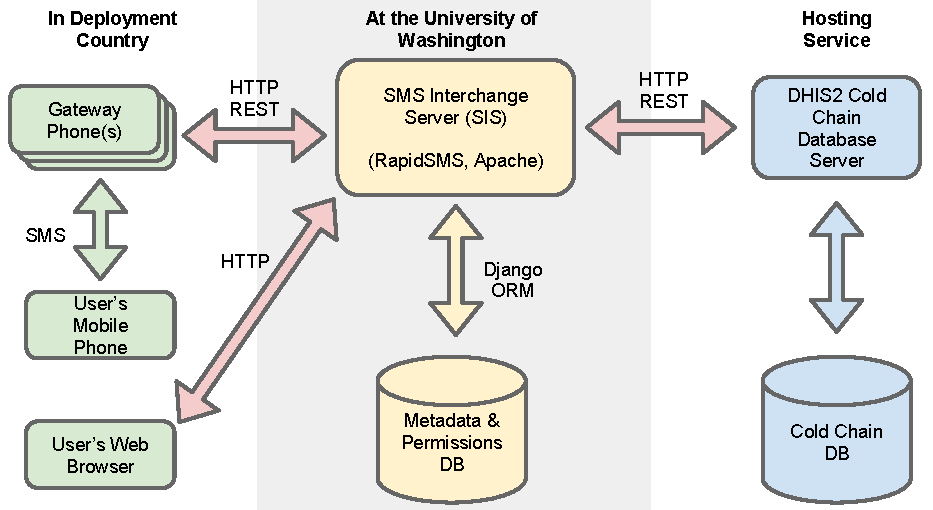
\epsfig{file=sim-broad-diagram.pdf}
\caption{SIM's relationship with other systems.}
\end{figure*}

SIM communicates exclusively via HTTP, which means it can be deployed on a wide range of web hosts. In order for CHWs to communicate with SIM via SMS, a ``gateway device'' must be deployed on the CHW's cellular network or a connected cellular network. The gateway device may be as simple as a midrange Android phone (the system was originally implemented using EnvayaSMS running on such a phone), or it may be as complex as a high-load dedicated gateway provided by the cellular provider. 

Although SIM was built to handle poorly-formatted SMS messages typed by hand by people with little access to training, there is no requirement that messages are hand-typed. The messages could just as easily be created by a simple application running on an embedded controller---for example, the FoneAstra system could automate data reporting by sending properly-formed SMS messages to SIM \cite{foneastra}.

The choice of where and when to use SMS and HTTP protocols was made carefully. The majority of users, especially CHWs reporting cold chain data, are without reliable access to Internet and power. This limits HTTP's usefulness. However, cell coverage in developing countries is good; recent estimates say that roughly five billion people in developing countries have access to a cell phone \cite{worldbank:mobileaccess}. SIM only requires several minutes of coverage per report and expects one or two reports per month, which we expect to be manageable.

However, SIM requires the gateway to have Internet access so that it may relay messages between SMS users and the SIM server. It also requires that moderators have Internet access. This allows SIM to provide a powerful, usable, bug-free moderation interface to review the system's operation.

In order to prevent malicious or accidental misuse, SIM only allows access from registered users (SMS users and moderators), each of whom is assigned one of several ``roles'' (with associated permissions). Among other things, privileged SMS users may register new users via SMS (for example, the facility manager would be able to register any other workers), and privileged moderators can access special tools for administering the Django and RapidSMS architectures on which SIM is based. This user information, which also includes each user's preferred language, is kept in a database managed by SIM.

However, SIM does not attempt to store any more cold chain information than necessary (typically only the facility hierarchy). Instead, SIM is intended to pass all of this data to a complete remote cold chain information/equipment management system such as DHIS2. That remote database is the permanent repository for cold chain data because it provides powerful querying and visualization tools (SIM does not, and is not intended to).

CHWs interact with SIM by sending structured SMS messages. Common use cases in Laos include

\begin{itemize}
\item A CHW periodically (monthly or more) sends one SMS message including both (a) their facility's current stock of each vaccine and (b) the number of times each of their fridges dipped below or rose above ideal temperature during the reporting period. Fridge data in Laos is recorded automatically by a Fridge-tag \textsuperscript{\textregistered} \cite{fridgetag}. If the CHW's message is too poorly-formatted to interpret, within several minutes a useful error message is returned (otherwise, a ``thank you'' message is returned). 
\item A facility unexpectedly runs out of stock of a particular vaccine, so a worker at the facility sends, as soon as possible, an SMS message identifying the vaccine. The stock outage is brought to the attention of the moderator the next time they log in so the outage can be handled rapidly. The same process can be used if any equipment fails.
\item It is a fact of life that workers come and go, change facilities, and change SIM cards. Privileged SMS users can register a new data reporter with a name, phone number, and associated facility by sending a single SMS message. Any worker can also change their preferred language at any time and see all SMS responses in that language.
\end{itemize}

Moderators interact with SIM by using a web application. Common use cases in Laos include

\begin{itemize}
\item Any incoming SMS messages that failed (for syntax or permissions reasons) are brought to the attention of a moderator. The notification persists in the moderation application until the moderator explicitly views and dismisses the source of the error. Errors are viewed in the context that sender's other messages, which allows moderators to track individuals and make informed decisions about how to handle a particular user's situation
.\item When viewing an SMS message with an error, a moderator can edit the message and resend it (internally, without incurring SMS charges) with any explicit permissions level. This gives moderators the power to quickly correct messages that the system cannot understand but a human can.
\item Moderators can view per-message logs of every side effect the message produced and each operation the system applied to the message (including parsing, verifying permissions, filtering for spam, etc.). This allows moderators to quickly identify bugs in the system and provide accurate and useful bug reports to developers.
\end{itemize}

We believe that SIM is the first step toward a powerful reusable framework for simple-to-deploy and simple-to-use SMS reporting systems.

\section{Related Work}

Using SMS operations to resolve failures in cold chain reporting is not a new idea. There are many projects, including research projects, commercial technologies, development frameworks, and extensions of existing software that address a similar problem. Many of these products have been deployed, and many have had more time to collect requirements and features than SIM has had.

However, SIM has several fundamental differences from these packages that make it a better solution if a programmer is available for several weeks to construct the SMS operations.

One solution is to use ``DHIS2 Mobile SMS Commands''. DHIS2 is a widely-used, powerful, open-source cold chain information/equipment manager. Because the SMS commands are supported on the same platform as the permanent data store, the integration between them is perfect. For example, the most up-to-date information about facilities and data is always available and any DHIS2 form can be turned into an SMS command. Furthermore, this module is meant to be used by non-technical staff, so new custom SMS operations with syntax and behavior can be configured through a web application. There are many behaviors, including scheduled notifications, data updating, listserves, and data queries. It is a powerful and complete solution \cite{dhis2:smsref, dhis2:smsoverview}.

However, the DHIS2 system has several limitations that SIM does not. First, it requires that DHIS2 is the deployment's permanent data store (however, the country may already be using a different solution or would prefer something a different one). Second, configuring SMS syntaxes in a web interface (SIM defines this in code instead) as DHIS2 does produces syntaxes that require careful delimiting with special characters (including the `+' and space characters), which is more difficult for data reporters to use. Third, there is little capacity to define custom actions or behaviors separate from what DHIS2 has implemented, so some behaviors may be impossible to obtain and others may be more complex than necessary. Finally, and perhaps most importantly, there is no way for moderators to see detailed logs of incoming SMS messages, especially ones that were rejected. This makes it difficult to diagnose common errors (fixing the syntax to reduce errors is be difficult as well) and identify particular people or facilities that require training \cite{dhis2:smsref, dhis2:smsoverview}.

In order to address syntax problems, DHIS2 publishes a Java Micro Edition (J2ME) application that can be installed on cell phones from many vendors (although DHIS2 recommends that the country buy and distribute a common device to provide better support and reliability). The application presents a user interface with input fields for the user to fill in, and then the phone produces a well-formatted SMS message to send to the server \cite{dhis2:smsoverview, dhis2:j2me}. This is an effective solution, but requires the country purchase and distribute dozens of hundreds of phones and to invest in both creating, deploying, supporting, and updating an application installed on those devices.

Another solution more similar to SIM is RapidSMS. In fact, SIM is based on RapidSMS, but with several key changes (which are discussed later, but whose motivations are discussed here). RapidSMS allows syntax and behavior to be described in code, just as SIM does. It's also written in the powerful Python language and based on a widely-used rapid web development framework called Django. This makes RapidSMS easy to customize and deploy. However, RapidSMS (and SIM by extension) requires programmers in order to implement new behaviors and syntaxes while other solutions can generate these based on configuration by non-technical users through a web interface. The RapidSMS XForms library attempts to mitigate this by allowing syntaxes to be defined in a similar way to DHIS2 (though with similar limitations), but not behaviors \cite{rapidsms:overview, rapidsms:xforms}.

SIM is a framework based on RapidSMS. While offering the same benefits as RapidSMS, particular ease of deployment and ease of customizing syntaxes and behaviors, SIM also provides two further benefits: 

\begin{itemize}
\item Looser coupling between operation syntax and behavior. RapidSMS suggests implementing policy decisions about behaviors (including updating remote databases, checking permissions, and more) in the same place as the syntax is defined. This means that changing a policy about behavior can require modifying code in many locations across many files. SIM, however, uses the observer design pattern to centralize and separate policy decisions so they can be modified or replaced easily in a single location without risking interfering with other behaviors.
\item A powerful and easily-integrated moderation interface. Any module that interacts with a message registers at least one ``effect'' in the database. The moderation interface merely displays these effects to the moderators. This both encourages developers to keep consistent, rich, and useful logs (in the form of these ``effects''), the benefits of which are well-known, and produces a minimal coupling between implementing new syntaxes/behaviors and integrating them into the moderation interface.
\end{itemize}

RapidSMS was the only framework that offered the flexibility that our requirements dictated, and even then it was not flexible or featureful enough to satisfy our requirements (especially because RapidSMS cannot allow multiple independent operations per SMS message, which we require). For that reason, we chose to implement a new framework. SIM has many advantages---it's easy to deploy, customize, and moderate as well as free to use and well-documented---that no single other framework provides.

\section{Approach}

The development of SIM has been guided by some basic design requirements: the system should support the SMS operations currently used by the prototype in Laos, it should be reusable and extensible enough to support a deployment in any other country. The intention for SIM is to design an open source system that will live on past this quarter. Ideally SIM will be extended, altered, and used by other groups in other countries, possibly even for purposes other than the cold chain distribution network. These requirements have guided the major design decisions including programing languages, frameworks, and documentation.

\subsection{Languages and Frameworks}

We selected the Python Django framework to create the web frontend and interface with a backend database that stores information needed for our system that is not part of the deployment country's health information system. This was an easy choice based on team members' familiarity with Django, its rich and diverse user base, and Django's use in the  RapidSMS framework (discussed later). New developers on this project that are familiar with Django will not have a problem getting started and those that are unfamiliar will have a wealth of resources from the Django community to help get them up to speed quickly. All of our server code is written in Python 2.7, which is commonly known among the development community and is very easy to learn. 
 
Because sending text messages between cell providers from different countries can be difficult and cost-prohibitive, we intend for the interaction with the server to be a RESTful HTTP interface. This decision was guided by the experience from the team working on the current prototype deployment in Laos. That design uses an Android device located in-country with an in-country phone number. All messages intended for the system are sent to that phone, and software on the phone forwards those incoming SMS messages to the server via an HTTP interface. It should be noted that this HTTP interface is a replaceable module. If another deployment requires a different interface a developer could easily write a new module for this purpose. 

As mentioned earlier, there are multiple software packages designed to handle incoming SMS messages and perform actions based on their contents. After a survey of various products we selected RapidSMS (as did the prototype project in Laos) because of its the well-defined phase-based handling of incoming messages and ease of developing specific message-handling modules. RapidSMS is also built with Django so it fits nicely with the other half of the system. The RapidSMS team has also taken special care to modularize the system with the intention that portions of the existing code would be implemented by developers deploying in different environments. The modularity of the HTTP interface was provided by the RapidSMS design and the HTTP backend used in our current working version (for EnvayaSMS) was reused from the prototype Laos project. While this choice of frameworks seemed right at the time, RapidSMS proved to introduce limitations that we hope to address with future work (discussed later). Whenever possible, SIM was designed to be as loosely coupled with RapidSMS as our development time permitted. Even if the implementation is replaced, the abstractions provided by RapidSMS are still valid and do contribute to SIM's design.

\subsection{Abstractions and Interfaces}

SIM's implementation is defined by two abstractions for ordering the execution of different modules and guaranteeing the side effects generated by the receipt of an SMS message. The first are the phases defined by RapidSMS that control the order of operations that are triggered when a message arrives. These phases in the order of execution are filter, parse, handle, and cleanup. Any registered app can act on a message at most once per phase and in any combinations of the phases. The second abstraction is the set of stages that we have defined for the side effects generated by a message. These stages are filter, syntax, semantics, commit, and respond. Note: the filter stage was created in direct response to the filter phase and their meaning is essentially the same. As a message passes through the RapidSMS phases it accumulates message effects that document a history of execution \cite{rapidsms:routers}. 

\begin{figure*}
\centering
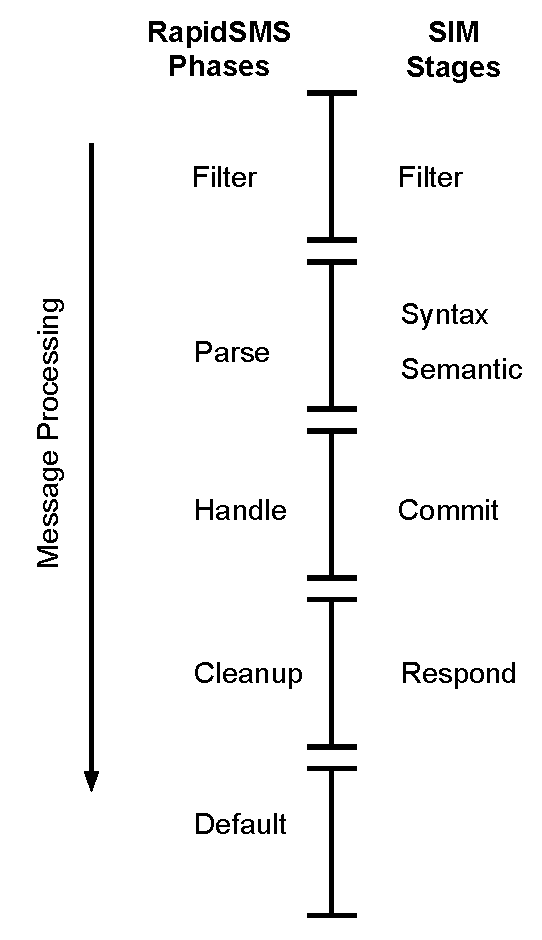
\epsfig{file=sim-stage-diagram.pdf}
\caption{RapidSMS phases compared to SIM stages.}
\end{figure*}

The SIM stages were designed to help log the side effects generated by the receipt of a message and in the event of a problem prevent future stages of execution on a message. For example, if the SIM server receives a malformed message the app that parses the message will attach an error (format discussed later) during the parse phase. Subsequently, any apps that act during the commit stage can be prevented from executing. This guarantees that side effects will not be generated on behalf of an invalid message. In this way, SIM ensures that untrusted data will not be saved to the database. Both the phases of operations and stages of side effects provide a useful division of actions and a way to deterministically guarantee the side effects caused by receiving a message.

Message Effects provide a form of communication between apps, and a mechanism for logging the processing of a message. The SIM stages defined previously dictate a history of when a Message Effect is created and the effects themselves are created with a defined type: 

\begin{description}
  \item[DEBUG] Debug effects are developer information of no relevance to users. \\
  \item[INFO] Info effects document successes or other non-errors. \\
  \item[WARN] Warning effects document minor or non-user actionable errors. Warnings are not typically returned to users, and do not prevent later processing from taking place. \\
  \item[ERROR] Error effects document user-actionable errors. Their messages may be returned to users and prevent later processing from taking place. \\
  \item[URGENT] Urgent effects are critically important information that must be seen and acted upon immediately. Their messages are always returned to users and do not halt further message processing. Use sparingly, if ever. \\
  \item[NOTIFY] Notify effects are critically important information that require human interventions and must be seen and acted upon by a moderator. Their messages are sent to moderators and do not halt further message processing. \\
\end{description}

Any app can create new Message Effects and attach them to a received message where they can be discovered by other apps that act upon the message later. The collection of Message Effects acts as an aggregation of knowledge that the installed apps have produced for an incoming message. The stage in which the message effect was attached and the type immediately communicate the nature of the effect and additional descriptive data can be included as well. This allows for all types of side effects to be decoupled from the parsing of a message and from each other. All effects attached to the message can be reviewed from the web based moderation interface. This is helpful for developers while debugging and for moderators in the event that a user is sending malformed messages.

\subsection{Architecture Summary}

All apps must either register for operation in during one or more of the RapidSMS phases or register interest in an app that does. The first group are referred to as RapidSMS apps. The second group act in the previously defined side effect stages and are referred to as SIM apps. This design decouples the parsing of a message from the semantic meaning and the external side effects. If a deployment country would like to use the same operation code format but store the reported data in a different database schema, they could simply replace the SIM app that connects to the database while keeping the RapidSMS apps that parse the operation codes.

Our RapidSMS apps act during the filter, parse, handle, and cleanup phases. We have implemented RapidSMS apps that perform specific actions like parsing all the the operations codes from a message or responding to message senders. We have also implemented a RapidSMS app for every operation code that we support for the Laos deployment. This allows for the system to be extremely malleable to the specific needs of a deployment country. The operation code apps simply parse the arguments for the operation codes that they are registered to handle. These RapidSMS apps can be shared or modified between deployments when their needs align or new apps can easily be written to handle operations that require a different structure in their argument string. As an example we implemented a stock level app that parses the arguments to the ``SL'' operation code. It expects to find an argument string made up of alternating alphabetic vaccine codes and numeric stock levels. The RapidSMS apps we have written for individual operation codes only perform syntactic checks and hence create effects during our syntax stage. They do not create any side effects that are visible outside of the context of the received message. This is by design to increase modularity so that the syntax defining apps can be reused by different deployments.
 
Our SIM apps are where the business logic is performed. For example, the semantic correctness of a message is determined by a SIM app after passing the syntactic checks of the RapidSMS apps. SIM apps are designed to perform operations like reads and writes to a database. These will mostly be deployment specific but through the use of a carefully designed interface they can be removed and replaced with minimal effort. For this project the SIM apps have largely been stubbed out with temporary methods as the specific database interactions will be the focus of future work.

The connection between RapidSMS apps and SIM apps is handled by a standard Django signal interface. SIM apps can register callback functions as listeners to the RapidSMS apps \cite{django:signals}. SIM apps can register different functions for different stages which allows for a cleanly packaged module of code that has a related purpose. As an example, a single SIM app for committing to a database can include a callback function for verifying the semantics of a request and a callback for performing the write to the database. The semantics callback will get executed during the RapidSMS parse phase, while the commit callback will get executed during the handle phase.

\section{Implementation}

\subsection{Integration with RapidSMS}

\subsubsection{Contact Management}

RapidSMS represents users that send and receive SMS messages using two Django models: Contact and Connection. Contacts contain information unique to an individual person, such as their name and preferred language. Connections represent the association between contacts (people) and communication mechanisms such as an SMS phone number, email address or IRC handle. Each Connection instance is associated with a Backend object, which indicates the programmatic mechanism by which messages are sent and received using that connection. Each connection also contains an identity field that stores a uniquely identifying string for that backend (e.g. a phone number, email address or username), as well as a foreign key to a Contact object. Thus, Contacts have zero or more associated Connections, and a Connection can be associated with zero or one Contact.

When a RapidSMS backend receives a message, it looks up the Connection instance that corresponds with the received message's backend and identity, or creates one if no such connection exists. This connection is attached to the message. If the connection references a Contact, then attaching the connection to the message also identifies the person that sent that message.

RapidSMS' user model allows multiple means of communication to be associated with a single contact, which is more general than what SIM requires since we expect each SMS user to have at most one unique phone number. However, RapidSMS' Connection and Contact models are very tightly coupled with their framework, and cannot easily be replaced with models better suited to SIM. As a result SIM makes use of the Contact and Connection RapidSMS models, but has added additional user models and invariants to adapt RapidSMS' design into one SIM can use.

First, SIM considers all Connection identities to be phone numbers. We also enumerate the set of all possible backends in the Django settings module, and impose the invariant that every Contact is always associated with a Connection from every backend, all of which have identical identities. This allows SIM to differentiate between SMS messages received via Envaya, the online message tester and the moderation backends, while also allowing a contact to have a single ``phone number'' attribute that is always changed atomically.

Second, SIM adds a ContactProfile model which stores additional information about each RapidSMS contact. Contact profiles have a one-to-one correspondence with Contact models, and are automatically generated whenever a Contact model is created. This profile contains SIM-specific information about contacts, including their facility affiliation and permissions role. These two models are presented as a single object in the moderation interface, as fields from both Contact and ContactProfile appear together in the edit contact web form.

Finally, SIM imposes the invariant that Connection models are immutable except for their contact field. The origin of messages received by RapidSMS is stored only in Connection objects, thus modifying a connection could destroy the phone numbers of historical messages. The addition of this invariant allows phone numbers to be re-assigned between contacts while also preserving the association between historical messages and phone numbers. Additionally, since historical messages store a reference to the Contact object they were associated with when they were processed, modifying a Connection's contact field does not destroy associations between historical messages and contacts.

\subsubsection{Message Processing}

\begin{figure*}
\centering
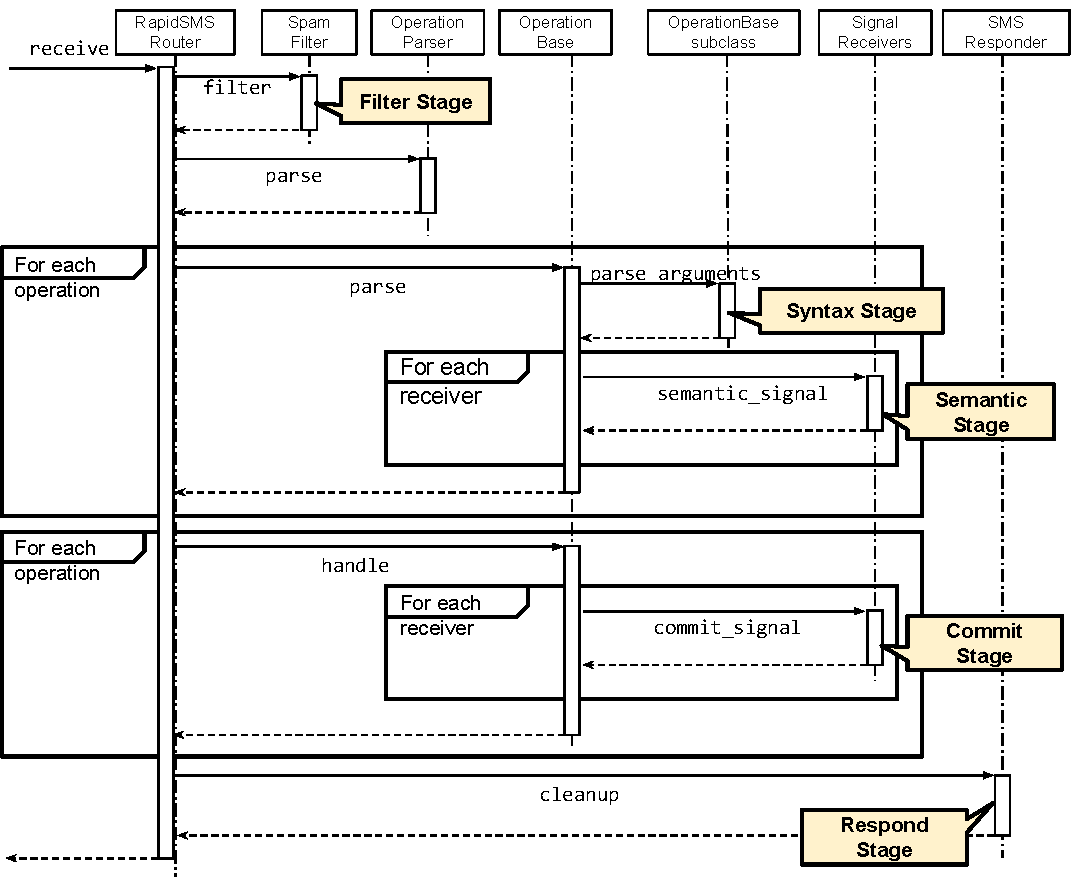
\epsfig{file=appendices/adapter.pdf}
\caption{RapidSMS/SIM Adapter Sequence Diagram}
\end{figure*}

RapidSMS and SIM make very different assumptions about the structure of incoming messages, and thus have very different message processing schemes. RapidSMS is based on the principle of each message containing a single operation, which is dispatched to and handled primarily by a single module. This module is responsible for most aspects of the message's processing, including parsing, semantic checks, side effects, and generating an SMS response. RapidSMS' phasing scheme reflects this: though some phases exist so that other modules can filter out spam (the filter phase) or add additional information such as a user's identity (the parse phase), only a single handle phase is intended to be executed for each message. More precisely, the first RapidSMS application that believes it can handle a message generally suppresses all other handlers by having its handle function return True to the router.

SIM is designed to allow an arbitrary number of operations in a single message. Thus, delegating the handling of a message to a single module is not possible, as every module that implements an operation could potentially have reason to handle part of a message. SIM's stages are designed to give all apps an opportunity to act at each stage, and adds an additional mechanism (Django signals) for modules to register interest in the semantics or side effects of an operation without defining the syntax of that operation.

The incompatibility of RapidSMS' message processing scheme with SIM's requirements did not become apparent until half way through the quarter. Since we deemed the risk of departing completely from RapidSMS's framework to be unacceptably high, we designed SIM to be implementable using RapidSMS' message processing scheme despite some incompatibilities between the two. Below is a description of each of SIM's stages, and how these stages are implemented using RapidSMS. Appendix 1 contains a UML sequence diagram that illustrates this implementation.

\paragraph{Filter Stage}

The filter stage gives apps an opportunity to halt further processing of the message. Currently only the spam filter makes use of the filter stage, in order to prevent processing of messages from unregistered phone numbers. SIM's filter stage is equivalent to RapidSMS's filter phase, thus filter stage handlers in our implementation are created by subclassing RapidSMS' AppBase class and overriding the filter method.

\paragraph{Operation Parser}

Though not a client-visible stage, the operation parser is a necessary step before the syntax stage can occur. This component is responsible for splitting the message into its constituent operations, and attaching this information to the message object before the Syntax stage. The operation parser does not interpret the arguments of each operation, it only identifies what substring of the message contains these arguments.

The operation parser is implemented in the RapidSMS parse stage, and is guaranteed to run before any Syntax stage application by being placed first in Django's list of installed apps. It uses a simple single-pass algorithm over the message that detects and splits on opcodes.

Some special parser behavior is necessary in order to avoid message ambiguity and common user errors:

\begin{itemize}
\item Some operations (HE and RG) take other opcodes or arbitrary strings as parameters. In order to avoid ambiguity when splitting these messages, such opcodes are required to appear at the end of a message. Any text beyond a HE or RG opcode is assumed to be part of the preceding operation's arguments, regardless of whether the text contains other opcodes.
\item Users unfamiliar with latin characters often confuse the character O with the numeral 0. In order to better interpret such messages, all O characters in a message are converted into zeros by the parser. Messages are also converted into uppercase to avoid case sensitivity. The RG opcode is configured to be an exception to these rules, as its arguments contain a user's name which is case sensitive and may contain O characters.
\end{itemize}

\paragraph{Syntax Stage}

In the Syntax stage, the arguments of each operation are parsed into a Python representation. If syntactic errors are reported for an operation, then that operation does not proceed to the Semantic stage, and no operations in that message proceed to the Commit stage.

The OperationBase class encapsulates all the behavior required to process a single type of opcode, and is responsible for implementing SIM's Syntax stage. An operation in SIM is defined by subclassing OperationBase and overriding the parse\_arguments method. This method is passed an opcode, unparsed argument string and message object, and returns a Python representation of the arguments of that operation. If an error is encountered while parsing the operation's arguments, parse\_arguments adds error effects to the passed message describing the failure.

The Syntax stage is implemented within RapidSMS' Parse phase. Each OperationBase is a subclass of AppBase, although subclasses of OperationBase do not directly interact with RapidSMS. At the beginning of its parse method OperationBase determines if its registered opcode (as defined in the project settings) appears within the message based on the output of the operation parser. For each matching operation, OperationBase calls parse\_arguments on that operation and attaches the returned Python arguments to the message.

\paragraph{Semantic Stage}

The Semantic stage verifies that an operation's arguments are valid. If semantic errors are reported for any operation, then no operations in that message proceed to the Commit stage. Clients of the semantic stage register interest in a particular operation using a Django signal. Whenever a message contains the registered operation, the signal receiver is passed the message object, opcode and Python arguments to the operation. Semantic signals are expected to return a list of message effects that indicate whether the message is semantically correct. If any semantic signal receiver returns an error effect, the message is flagged for moderator review and the commit stage is not allowed to proceed.

SIM's Semantic stage is implemented in OperationBase's parse method. After calling parse\_arguments for a particular operation and verifying that no syntactical errors exist, OperationBase then fires the semantic signal for that operation. The effects returned by the signal receivers are then finalized and saved in the database.

\paragraph{Commit Stage}

The Commit stage performs any side effects (for example, updating a local or remote database). The purpose of previous stages is to guarantee that the Commit stage will succeed for all operations. Like the Semantic stage, clients of the Commit stage can register interest in a particular operation using a Django signal. They are passed the same arguments as the Semantic signal, and return message effects indicating the outcome of their side effects.

SIM implements the Commit stage during RapidSMS' Handle phase, by overriding the handle method of OperationBase. First, if any errors are detected from previous stages, OperationBase halts without performing any commits. Otherwise, for each matching operation in the message OperationBase fires the commit signal for that operation. The effects returned by the signal receivers are then finalized and saved in the database.

OperationBase's handle method always returns False, in order to allow all operations an opportunity to handle the message.

\paragraph{Respond Stage}

This stage gives apps (though typically only one) an opportunity to aggregate the logged message effects and send a response to a user. It  is equivalent to RapidSMS's Cleanup phase, thus Respond stage handlers in our implementation are created by subclassing RapidSMS' AppBase class and overriding the cleanup method.

SIM's current implementation of a responder module sends back all urgent message effects to the user, and selects the first error effect not appearing in the commit stage to send as well. Error effects from the commit stage are not returned to users, as these are generally not user-actionable. If no errors require a response, a generic ``thank you'' response is sent.

\subsubsection{Miscellaneous Integrations}

Several other miscellaneous integration details are worthy of mention:

\begin{itemize}
\item RapidSMS routers were designed with the assumption that a single RapidSMS app exists for each Django application. More precisely, each Django app is expected to contain an ``app'' submodule containing a single declaration of an AppBase subclass. Since we group multiple operations (each of which is an AppBase subclass) in a single Django module, SIM must bypass RapidSMS' auto-discovery of AppBases and directly insert OperationBase subclasses into the RapidSMS router. This is performed in the project's settings module.
\item SIM makes use of RapidSMS' messagelog application, which logs every message sent or received by RapidSMS as a Django model. However, RapidSMS' implementation only logs messages that pass the Filter phase. Since filtered message may contain valuable information (such as an unregistered user's attempts to submit data), we modified the messagelog application to log messages in the beginning of the filter phase instead of the parse phase.
\end{itemize}

\subsection{Permissions}

Permission checks are implemented in SIM's semantic stage, by registering functions with an operation's semantic signal. SIM's current permission model assigns a role to each contact, which dictates which opcodes that contact is allowed to use. The entire permissions policy is contained in a single module for ease of modification when SIM is used by different countries.

\subsection{Moderation Web Interface}

The moderation web interface is implemented as a typical Django web application. Regular expressions are used to dispatch a request's URL to a view function, which is passed the request and returns a response to be sent back to the web client. Views that return an HTML page use Django's templating language to separate business logic (in view functions) from rendering logic (in templates). Numerous other Django features such as the form library, session management, authentication, CSRF tokens and clickjacking protection are also used by SIM.

The layout of the moderation interface is implemented using the Twitter Bootstrap UI framework, which in turn makes use of the jQuery JavaScript framework. These frameworks allow us to create elegant, mobile-responsive web pages quickly and efficiently, and ensure a consistent look-and-feel throughout the moderator interface. A third-party library (django-crispy-forms) was also used to better integrate Django's form rendering with bootstrap.

\subsection{Internationalization}

A key requirement for SIM is that all content delivered to a user must be in a language they understand. As a result, virtually every part of SIM's implementation makes use of Django's internationalization framework to identify and translate strings that are visible to users. Django's framework makes use of the GNU gettext tools, and implements many of gettext's functions in Python for use by Django developers. In general these functions take a string as input, and return a translation of that string in some form.

In addition to implementing runtime translation of strings, translation functions are used by a code analysis tool to automatically detect strings that need to be translated, and generate appropriate translation files that map English strings to translated strings. These files are loaded by Django at startup to build in-memory data structures that are used to implement efficient translation.

The selected language of a web user is stored within their session, and is activated by a Django middleware class before a view function is called. Python strings that are evaluated within view functions are wrapped in immediate translation functions (ugettext and ungettext), which return the translated value of that string. Immediate translation functions are also used by Django's template language in order to implement the trans and blocktrans template tags, which are used throughout the moderation site templates.

When sending SMS responses, the recipient's preferred language is determined using the associated Contact instance. After this language is activated, immediate translation functions are used just like in a Django view function or template.

Some Python string literals must be initialized before a user's language can be activated. For example the models and settings modules of a Django project are loaded before they are used in a view function or SMS response. In these cases lazy translation functions (ugettext\_lazy and ungettext\_lazy) are created instead of immediately translating the string. These functions return lazy objects that evaluate to translated strings when accessed in a way that requires knowledge of their value, which typically occurs when the string is converted to unicode when rendering a template or SMS message.

Internationalizing the names and descriptions of message effects is more complex, since they are displayed in multiple languages after being inserted into SIM's database. We decided to represent these strings using two database fields: an English format string and a JSON dictionary that maps replacement fields to string values. Format strings that are inserted into the database are wrapped with a ``noop'' translation function (ugettext\_noop) which does not modify the string's value, but indicates to the code analysis tool that the contained string must appear in translation files. When an effect's name or description are retrieved from the database they are wrapped in lazy translation objects which are evaluated after the appropriate user language is activated.

Our implementation of internationalized message effects has some limitations. Translated strings cannot be nested, which complicates the creation of message effects that aggregate other effects. Implementing the SMS responder application highlighted these limitations, as the responder needed to log which effects were sent in response to a message without being able to reference the names or descriptions of those effects it its own logged effects. This specific problem was addressed by adding a field to message effects that indicates if they were selected to appear in a response, however in general composing message effects is not possible.

A possible solution is to create a JSON representation of translation strings that is recursive. A translation object would consist of a format string and dictionary mapping replacement fields to values. Each field value is either a string or a nested translation object with its own format string and field mapping. This would allow translation objects to be composed, but falls outside of Django's translation best practices and would require additional specification and testing. This improvement was not implemented this quarter due to time constraints.

\section{Evaluation}

\subsection{Importance of Generalizability}

While our project was mainly based on requirements for a deployment in Laos, we also designed SIM to be easily adaptable for use by other countries. Thus, one of the key features of our project was that it had to be easily generalizable and scalable. The core challenge in implementing SIM to be generalizable was designing the system to be decoupled enough to allow different components to be customized and easily swapped out for different deployments. Building our project as a series of apps, and designing different operation codes to be handled by their own app, allows future developers to easily swap out operation codes as well as the permissions system. Our project was also built without reliance on a particular backend database to accommodate deployments for different operations that may not use DHIS2.

In order to further understand the necessary requirements for a more general system, we spoke with several health center representatives from other international organizations such as UNICEF, PATH, and VillageReach, which proved to be very useful in outlining general use cases across different organizations. One of the main takeaways from our conversations with these representatives was learning more about the kind of technical and physical environments where our system will be used, and the current inefficiencies in the cold chain and existing reporting systems that our new system should try to avoid. This knowledge allowed us to understand what specific components of our system were crucial to increase the efficiency of the cold chain, and allowed us to rank features by degree of importance for our baseline implementation.

Our work thus far has been focused on building a system to be deployed for health facilities in Laos, where a prototype of our system is already in place. We used feedback from health workers in Laos who are currently using the prototype to understand adaptations that would need to be made in our system. In addition, we demoed SIM for various health center representatives. During these demos, we walked them through the moderation interface to demonstrate a typical use of our system from a moderator's perspective, and provided a technical overview and explanation of the different Message Effects and message processing stages employed by SIM. Based on our conversations with these health organization representatives, as well as the feedback from Laos health workers using the prototype of our system, the three main criteria for usability that we used to evaluate our project was that our system had to be easy to use, provide up to date data, and provide clear and unambiguous error messages.

\subsection{Clear and Easy to Use}

The results of initial use of the prototype in Laos and the logs generated for text messages sent by community health workers to our system confirmed that in order for our system to be easy to use, SIM would need to have a robust SMS message parser. One finding from the use of the Laos prototype was that users who are not familiar with latin characters found it difficult to distinguish between ``o'' and ``0'' or ``S'' and ``\$'' when typing SMS messages. Given that these characters are heavily used in both operation codes and vaccination codes, our parser had to be able to understand messages that contained such errors and continue to parse them. It was also important for the parser to be able to ignore random spacing between characters as well as random punctuation characters between input, as these extraneous characters were also found in the SMS logs generated by health workers testing out the Laos prototype. Building a parser that could gracefully handle these errors and continue normal parsing of the message was crucial to allow for users unfamiliar with English to use our system without immense frustration due to typos.

A second consideration for building a system that would be clear and easy to use involved the ability to customize language settings. Health workers in Laos had trouble understanding the English romanticization of Laotian words. While most health workers could read Thai characters, we were unable to use Thai characters in our system for political reasons. Thus, our system allows users to set their language preference to English, Karaoke, or Lao. Based on our conversations with health organization representatives, allowing a user to switch between viewing the application in English and their native language is important outside of Laos as well, due to the fact that many technical terms, such as the names and identifiers for various vaccines, are often in English.

\subsection{Providing Up-to-Date Data}

It is crucial to have up-to-date data about stock levels and equipment failures for both health centers and patients. Patients need to know if a health center has enough vaccine stock before making the trip to a health facility to be vaccinated. In some areas, making the trip to a health facility can be very difficult and time consuming. A patient who travels a far distance to be vaccinated only to find that the health facility is out of stock may not be willing to risk such an incident occurring again if they were to re-visit the facility at a later date. Such disappointments damage the trust between health facilities and patients. Health center workers and district level managers also need to be notified as soon as possible of equipment failures so that they can dispatch technicians as well as salvage as many vaccines as possible in the meantime. Because our project has not yet been integrated with DHIS2, we were unable to evaluate our project based on this criteria for this iteration of the implementation of SIM.

\subsection{Unambiguous Error Messages}

When sending text messages to the system, health workers may sometimes forget that they are interacting with a server rather than a human being. According to one health representative, sometimes a health worker using an SMS-based reporting system sends a text message containing typos and receives a text message from the server stating simply that the text message was improperly formatted, without information about what was wrong with the formatting of the sender's original message. However, in some cases, the health worker tried to respond to this message by asking for details about the errors in the original message, or sent the same message again. In order to prevent this and prevent potential user frustration, our system aims to provide moderators with both in-depth feedback about errors as well as information about which SIM stage the error occurred in when processing the incoming message, and aims to provide the user with a clear error message as well as the ability to ask for information about the usage of a particular operation code.

\section{Conclusion and Future Work}

\subsection{Lessons Learned}

The most difficult part of the design and implementation of SIM by far was gathering requirements for the system, and designing SIM to accommodate all of the requirements specific to the Laos deployment without sacrificing generalizability or scalability. We found that it was important to gather requirements for our system as early as possible, as it was impossible to finalize our architecture design due to newly discovered requirements or previously unforeseen constraints.

\subsection{Next Steps for Laos Deployment}

\subsubsection{Localization}

Translations of error messages and other Message Effects strings, messages sent to the user, and strings used in the web interface are also needed before SIM can be deployed to Laos. To this end, our group has contacted a translator who has offered to help us translate the necessary strings from English into Lao, and these translations are currently underway.

\subsubsection{DHIS2 Integration}

The first major component that needs to be completed for the Laos deployment is integrating the existing project with the DHIS2 backend used by health facilities in Laos so that data reports can be periodically committed to DHIS2. This would involve implementing handlers for commit signals to send or retrieve data from DHIS2 as part of SIM's commit stage.

\subsubsection{User Reminders}

Sending reminders to users on a regular basis to ensure timely reporting of data about the cold chain is another important next step for the Laos deployment. This would involve sending SMS messages to data workers who have not submitted monthly reports until these reports are submitted, at a frequency determined by administrators. 

\subsubsection{Spam Filter Improvements}

One suggestion that we received from feedback on a recent demo of SIM was to allow the spam filter to send a response to the user if their message was filtered due to an unrecognized number. Currently the spam filter logs the message and halts all processing of the message if the sender is not a recognized health worker or administrator, but does not send any response back to the sender. Sending a response to spam messages would be helpful in notifying health workers as soon as possible if they are not registered in the system so that they do not make the mistake of submitting reports before they are properly registered. 

A malicious user, however, could potentially waste funds by sending numerous SMS messages to the system, and should be blocked. It would be useful to have a way of distinguishing between malicious spammers and unregistered users by determining if the same unrecognized user is trying to send an inordinate number of messages. A more advanced filtering stage may also be useful for the detection of automatic response loops that potentially drain funds. Thus, it would be helpful to have a way to keep track of the number of messages sent by and to each user in the system. Keeping track of these counts would also be helpful for facilities in determining how much to reimburse health workers for sending and receiving SMS messages using their personal phones.

\subsubsection{Customizeable User Roles}

It would also be beneficial to allow for moderators to have more flexibility in customizing health worker roles and the operation codes that each user is allowed to submit via SMS. Currently, only two roles exist to represent the list of operation codes associated with administrators and data reporters, but the list of permitted operation codes has been hard-coded as part of the SIM project settings file. Allowing administrators to adjust these roles in a non-programmatic way would increase the adaptability of our system to potential future changes in the hierarchical structure of facility workers.

\subsubsection{Improved Error Messages}

As discussed in the Evaluation section, it is very important to ensure that error messages and logged Message Effects contain useful information for both users and moderators that is easy to understand. All Message Effect text strings should be evaluated for their helpfulness in explaining the context of the Message Effect to the relevant user, and improved where necessary. 

One interesting case to note is that if a user sends a batch of SMS messages in rapid succession, some of which contain errors, the user will get a batch of SMS responses back from SIM, but may not be able to deduce the original text message that each response is associated with if some of these responses contain reports of syntactic or semantic errors. This kind of ambiguity in the logged error messages makes it difficult for a user to correct errors in their SMS reports. It may be useful to consider including more detailed information about the context of the original text message, so that a user can clearly identify the SMS reports that were successfully received, and those that need to be resent.

Thus, in addition to the technical improvements described above, it would be useful to meet with and demo our project for health workers, administrators, and other representatives from various health organizations located in and outside of Laos to gain more feedback on the perceived usability of our system, as well as the look and feel of the moderation interface.

\subsection{Potential Directions for Future Work}

\subsubsection{Querying DHIS2}

Providing managers at the district and national levels with the ability to query the DHIS2 database for information regarding equipment status and stock distribution could help administrators to better assess the efficiency of the cold chain. An example use case is that such a querying system could allow managers to do analysis for a particular country and get information about how well each level of the cold chain is working. Receiving a high-level overview or comparison of the performance of various health facilities would help managers to pinpoint sections of the cold chain or specific facilities that are inefficient, and allow these managers to assess the frequency of failures and discover the reasons behind poor performance in such facilities. Thus, it would be useful for a district or national level manager to be able to send an SMS message asking about aspects of the cold chain such as equipment failures, equipment shortages, stock overflow or distribution levels, and receive a reply summarizing this information across multiple facilities for easy comparison and review.

\subsubsection{Location Information}

In addition to allowing district or national level managers to query the DHIS2 database, another potential direction for future work would be to include or make use of existing location information stored in DHIS2 to allow health workers in the field to query the database. One possible use case would be to allow a health worker out on an outreach trip to provide vaccinations at a nearby village or town, or perhaps even a patient who is looking to be vaccinated, to send an SMS asking for information about the nearest facilities such as location, hours, and current vaccine stock levels. Adding this ability would also aid in vaccine redistribution in cases where a facility has too much or too little stock. The ability to access accurate and up-to-date data about the stock levels at other facilities would allow facilities to communicate more efficiently with each other and collectively work to deal with stock outages and prevent waste. This feature would also help to build patient trust in the ability of the health center to meet their needs, especially for patients who may need to travel far distances just to reach the health center. Such patients could send an SMS to the system to ask for the nearest locations where they have the best chance of receiving a vaccination.

\subsubsection{Alternatives to RapidSMS}

RapidSMS was designed to handle SMS messages that contain a single operation code, and the phases and message handlers defined for the RapidSMS router are not sufficient for dealing with messages that deal with messages containing multiple operation codes that may also depend on each other. The main benefit of RapidSMS is that the router is a convenient middleman between RapidSMS apps and the backend. However, one possible area for future work is to replace the RapidSMS router with a customized router implementation of our own to accommodate the more intricate stages for checking syntax, committing data, and responding to users that our system requires. 

\subsubsection{Improving the Operation Parser}

The current implementation of the delimiter-based parser for incoming SMS messages to our system created extra requirements when defining operation codes because the delimiter-based approach meant that vaccine names or other strings that contained operation codes may be misinterpreted as representing actual operation codes. Thus, it may be beneficial to explore alternative implementation strategies for the parser, such as the possibility of a parser that is based on context free grammars and has some knowledge of the associated grammatical patterns for the arguments required for submission with each operation code

In short, the SMS Immunization Manager (SIM) is a system designed to improve the efficiency of vaccine cold chains. We have built the foundation for a system that will provide health workers with an easier and more reliable way of reporting vaccine stock levels and the status of crucial equipment, in order to replace the current cumbersome paper-based reporting system. There is a great need for timely and accurate reports in order to facilitate the efficient distribution of vaccines across health centers within a country. While this project was built with Laos specific requirements in mind, SIM was designed to be easily customized and scaled in order to be deployed for use in aiding the management of vaccine cold chains in other countries as well.  

\section{Acknowledgements}

We would like to thank Profs. Richard Anderson and Ruth Anderson for organizing CSE 481, providing us with a project to build, gathering requirements for our project, and connecting us with users and others who could provide feedback on SIM. We would also like to thank Trevor Perrier and Fahad Pervaiz for gathering requirements in Laos, implementing and deploying a valuable prototype, and taking over the project after CSE 481. We would also like to thank Ron Pankiewicz from VillageReach, who met with us twice to help define SIM's requirements and to provide feedback; Rajit Dhiman, who helped define requirements; and Lee, the IT administrator in for the Laos health ministry, who provided valuable feedback.

\bibliographystyle{abbrv}
\bibliography{report}  
\balancecolumns

\appendix
Many additional materials are available in our public code repository, on GitHub as ``ireynolds/sms-immunization-manager''. A comprehensive documentation site, which can be built and previewed using the nanoc static site generator, is available in the repository in the website/ directory.

\end{document}
